\documentclass[twocolumn, a4paper]{article}
\usepackage{indentfirst}
\usepackage{setspace}
\usepackage{amsmath}
\usepackage{algorithm}
\usepackage{algorithmic}
\usepackage{graphicx}
\usepackage{ctex}

\usepackage{amssymb}
\setlength{\parindent}{2em}
\title{\bf{Machine Learning SVM Report}}
\author{Hanwen Liu 522030910109}
\begin{document}
\maketitle
\section{Algorithm}

\subsection{Classic SVM Problem}
The SVM algorithm is invented to solve the classification problem with linear classifier. The classification can be described as: Given $N$ training data points:
\begin{equation}
\nonumber
  x_1,...,x_i,...,x_N \in R^m
\end{equation}
each with a label of
\begin{equation}
\nonumber
  d_i=+1\ or\ d_i=-1
\end{equation}
find a hyperplane
\begin{equation}
\nonumber
  w^Tx+b=0\ (w\in R^m, b\in R)
\end{equation}
which separates data into two groups:
\begin{equation}
\nonumber
  \{x_i|d_i=+1\}\ and\ \{x_j|d_j=-1\}
\end{equation}
As shown in figure \ref{fig:SVM},
\begin{figure}[htb]
  \centering
  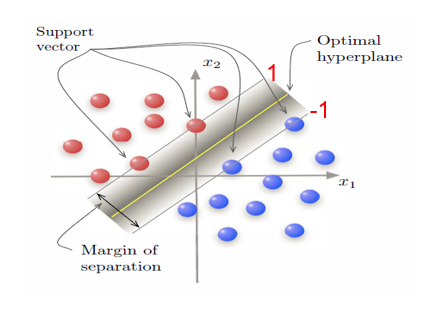
\includegraphics{SVMpng.png}
  \caption{SVM}
  \label{fig:SVM}
\end{figure}define the support vector as $x_p$ and $x_n$ and the vector on the hyperplane as $x_0$, we have:\begin{equation}
\left\{
\begin{aligned}
\nonumber
&w^Tx_p+b=1\\
&w^Tx_0+b=0\\
&x_p=x_0+\frac{w}{||w||}\dot \gamma
\end{aligned}
\right.
\end{equation}
We can derive from the above equations that the distance form the support vector to the hyperplane:
\begin{equation}
\nonumber
  \gamma = \frac{1}{||w||}
\end{equation}
Since the goal of SVM is to maximize the margin of separation and the margin of separation $\rho \propto \gamma$. Hence, the SVM problem can be formulated as:
\begin{equation}
\begin{aligned}
\nonumber
  min\ &\frac{1}{2}w^Tw\\
  s.t.\ &d_i(x_iw+b)\ge 1\ i=1,2,...,m
\end{aligned}
\end{equation}
It's Lagrangian function is:
\begin{equation}
\nonumber
  L: \frac{1}{2}w^Tw-\sum_{i=1}^N\alpha_i[d_i(x_i^Tw+b)-1]
\end{equation}
From the KKT condition, we can obtain its dual problem:
\begin{equation}
\begin{aligned}
\nonumber
  max:\ &\sum_{i=1}^N\alpha_i-\frac{1}{2}\sum_{i=1}^N\sum_{j=1}^N\alpha_i\alpha_jd_id_jx_i^Tx_j\\
  s.t.\ \ &\alpha_i\ge 0,\ \sum_{i=1}^N\alpha_id_i=0
\end{aligned}
\end{equation}

\subsection{Slack Variable}
In various situation, the ideal hyperplane may not exist since the data is not linearly separable. Hence, slack variable $\xi$ is introduced to optimize the original SVM problem as shown in figure \ref{fig:sla},
\begin{figure}[htb]
  \centering
  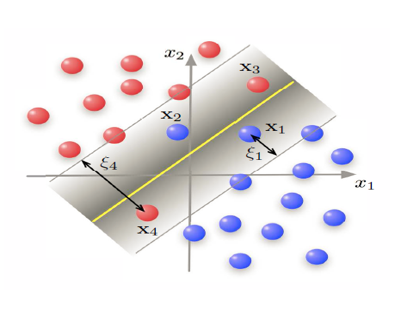
\includegraphics{slack.png}
  \caption{Slack Variable in SVM}
  \label{fig:sla}
\end{figure}
Then the original problem can be written as:
\begin{equation}
\begin{aligned}
\nonumber
  min\ &\frac{1}{2}w^Tw+C\sum_{i=1}^N\xi_i\\
  s.t.\ &d_i(w^Tx_i+b)\ge 1-xi_i\\
  &xi_i\ge 0
\end{aligned}
\end{equation}
Applying the Lagrangian function and KKT condition, we can obtain its dual problem
\begin{equation}
\begin{aligned}
\nonumber
  max:\ &\sum_{i=1}^N\alpha_i-\frac{1}{2}\sum_{i=1}^N\sum_{j=1}^N\alpha_i\alpha_jd_id_jx_i^Tx_j\\
  s.t.\ \ &\sum_{i=1}^N\alpha_id_i=0\\
  &0\le \alpha_i\le C
\end{aligned}
\end{equation}
where $C$ is set by user to control the trade-off between a large margin and a small error penalty.

\subsection{Sequential Minimal Optimization}
The SMO algorithm is introduced to solve the SVM dual problem. The dual problem is to maximize\begin{equation}
\nonumber
  \sum_{i=1}^N\alpha_i-\frac{1}{2}\sum_{i=1}^N\sum_{j=1}^N\alpha_i\alpha_jd_id_jx_i^Tx_j
\end{equation}
The aim is to obtain each $\alpha_i$ to maximize the goal. The idea is that: iteratively select $\alpha_i$, $\alpha_j$ and fix other $\alpha$ to optimize $\alpha_i$, $\alpha_j$ until no optimization can be applied to any $\alpha$.\\
Before the explanation, we should introduce kernel first. As shown in figure \ref{fig:hig},
\begin{figure}[htb]
  \centering
  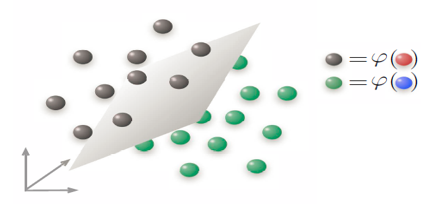
\includegraphics[width=0.5\textwidth]{high.png}
  \caption{Increase Dimension}
  \label{fig:hig}
\end{figure}
sometimes non-lineary-separable patterns may be transformed into a new feature space in which they are linearly seperable.\\
There we introduce the transformation $\phi$. Then the dual probelm can be expressed as
\begin{equation}
\begin{aligned}
\nonumber
  max:\ &\sum_{i=1}^N\alpha_i-\frac{1}{2}\sum_{i=1}^N\sum_{j=1}^N\alpha_i\alpha_jd_id_j\phi^T(x_i)\phi(x_j)\\
  s.t.\ \ &\sum_{i=1}^N\alpha_id_i=0\\
  &0\le \alpha_i\le C
\end{aligned}
\end{equation}
Kernel is introduced here so that we can combine $\phi^T(x_i), \phi(x_j)$
\begin{equation}
\nonumber
  K(x_i,x_j) = K(x_j,x_i)=\phi^T(x_i)\phi(x_j)=\phi^T(x_j) \phi(x_i)
\end{equation}
The frequently used kernel includes linear kernel, polynomial kernel, gaussian kernel and sigmoid kernel.\\
Now suppose we choose $\alpha_1$ and $\alpha_2$ to optimize and fix other $\alpha$. Then the problem can be formulated as
\begin{equation}
\begin{aligned}
\nonumber
  max\ &W(\alpha_1,\alpha_2) = \alpha_1 + \alpha_2 - \frac{1}{2}K_{1,1}d_1^2\alpha_1^2-\frac{1}{2}K_{2,2}d_2^2\alpha_2^2\\&-K_{1,2}d_1d_2\alpha_1\alpha_2-d_1\alpha_1\sum_{i=3}^N\alpha_id_iK_{i,1}\\&-d_2\alpha_2\sum_{i=3}^N\alpha_id_iK_{i,2}+C \\
  s.t.\ \ &\alpha_1d_1+\alpha_2d_2=-\sum_{i=3}^N\alpha_1d_i\\
  &0\le \alpha_1, \alpha_2\le C
\end{aligned}
\end{equation}
Then, we have
\begin{equation}
\begin{aligned}
\nonumber
  \frac{\partial W}{\alpha_2} = &-(K_{1,1}+K_{2,2}-2K_{1,2})\alpha_2^{new}+(K_{1,1}+K_{2,2}\\&-2K_{1,2})\alpha_2^{old}+d_2[d_2-d_1+f(x_1)-f(x_2)]
\end{aligned}
\end{equation}
where $f(x)=\sum_{i=1}^N\alpha_id_iK(x_i,x)+b$\\
Denote $E_i=f(x_i)-d_i$ and $\eta = K_{1,1}+K_{2,2}-2K_{1,2}$, we have
\begin{equation}
\nonumber
  \frac{\partial W}{\alpha_2} = -\eta \alpha_2^{new}+\eta \alpha_2^{old}+d_2(E_1-E_2)=0
\end{equation}
which leads to 
\begin{equation}
\nonumber
  \alpha_2^{new}=\alpha_2^{old}+\frac{d_2(E_1-E_2)}{\eta}
\end{equation}
Since $\alpha_1$ and $\alpha_2$ should satisfy the constraint, so $\alpha_2^{new}$ needs to be clipped as
\begin{equation}
\alpha_2^{new}=\left\{
\begin{aligned}
\nonumber
&H\ &\alpha_2^{new}>H\\
&\alpha_2^{new}\ &L\le \alpha_2^{new} \le H\\
&L\ &\alpha_2^{new}<L
\end{aligned}
\right.
\end{equation}
where $L,H$ are defined as:\\
when $y_1 \ne y_2$
\begin{equation}
\left\{
\begin{aligned}
\nonumber
&H = min(C,C+\alpha_2^{old}-\alpha_1^{old})\\
&L = max(0,\alpha_2^{old}-\alpha_1^{old})
\end{aligned}
\right.
\end{equation}
when $y_1 = y_2$
\begin{equation}
\left\{
\begin{aligned}
\nonumber
&H = min(C,\alpha_2^{old}+\alpha_1^{old})\\
&L = max(0,\alpha_2^{old}+\alpha_1^{old}-C)
\end{aligned}
\right.
\end{equation}
Therefore, we can optimize $\alpha_1$
\begin{equation}
\nonumber
  \alpha_1^{new}=\alpha_1^{old}+d_1d_2(\alpha_2^{old}-\alpha_2^{new})
\end{equation}
Also, we can update $b$
\begin{equation}
b^{new}=\left\{
\begin{aligned}
\nonumber
b_1=&-E_1-d_1K_{1,1}(\alpha_1^{new}-\alpha_1^{old})-d_2K_{1,2}\\&(\alpha_2^{new}-\alpha_2^{old})+b^{old},\ 0<\alpha_1^{new}<C\\
b_2=&-E_2-d_1K_{1,2}(\alpha_1^{new}-\alpha_1^{old})-d_2K_{2,2}\\&(\alpha_2^{new}-\alpha_2^{old})+b^{old},\ 0<\alpha_2^{new}<C\\
b_3=&\frac{1}{2}(b_1+b_2),\ otherwise
\end{aligned}
\right.
\end{equation}
The SMO algorithm is done by iteratively updating every $\alpha$ and $b$ until no change can be done. In my SVM algorithm, SMO is done for fixed times which is controlled by user to control the trade-off between efficiency and accuracy.
\subsection{SVM On Multiple Classes}
The classic SVM focus on classification between two classes, which prevents the application of SVM directly in the classification problem between more than two classes. Therefore, some updates need to be done to better the algorithm to suit more complex situations such as CIFAR-10 and MNIST.\\
The strategy used here is to train a number of SVM model and apply every one of them on a $x_i$ to correctly find its label. For example, we have a dataset with $3$ labels, then $3$ SVM models will be trained to classify data between label $1$ and  label $2$, label $1$ and label $3$, label $2$ and label $3$.\\
To predict the label of $x_i$, we need to apply the 3 trained models on $x_i$ and count the number of predicted label. If label $2$ is predicted twice and label $1$ is predicted only once, than the overall prediction is label $2$ since the number of label $2$ is larger than the number of label $1$.\\
We 
\\Similarly, the data has $k$ labels. Then we should train $C_k^2$ SVM models and than apply each of them on a data and count the number of each label to find the largest one be the outcome.

\subsection{Multiple Kernel In SVM}
Sometimes single kernel SVM performs badly when the features of the data are highly complex, so a combination of multiple kernels are introduced to transform the data into a linearly separable feature space where single kernel can not transform. It can be expressed as
\begin{equation}
\nonumber
  K_{i,j}^{mul} = \sigma_1K_{i,j}^{1}+\sigma_2K_{i,j}^{2}+...+\sigma_nK_{i,j}^{n}
\end{equation}
where $K^i$ means the type of $i$-th kernel (linear, polynomial...). The aim is to find the coefficient $\sigma_i$ of each kernel.\\
Consider a situation where the mixed kernel consists of two kernel $K_1$ and $K_2$ with their coefficients $\lambda$, $1-\lambda$ and their mapping function $\phi_1(x), \phi_2(x)$.\\
In the feature space, the distance of $x_i$ and $x_j$ is 
\begin{equation}
\nonumber
  d=||\phi(x_i)-\phi(x_j)||
\end{equation}
In classification problem, we hope to maximize $d$ between different labels and minimize $d$ between the same label.
\begin{equation}
\left\{
\begin{aligned}
\nonumber
&max\ d,\ d_id_j=-1\\
&min\ d,\ d_id_j=1 
\end{aligned}
\right.
\end{equation}
Expand $d$ with $K^1_{i,j}$ and $K^2_{i,j}$, we have
\begin{equation}
{
\begin{aligned}
\nonumber
&d(\lambda)=A\lambda^2+B\lambda+C\\
&M=K^2_{i,i}+K^2_{j,j}-2K^2_{i,j} \\
&A=M-2K^1(i,j)+2\\
&B=-2M\\
&C=M
\end{aligned}
}
\end{equation}
Therefore, we can define the evaluating function $L(\lambda)$
\begin{equation}
{
\begin{aligned}
\nonumber
  max\ L(\lambda)&=\sum_{i}^N\sum_{j=1}^{i-1}d(\lambda)|_{d_id_j=-1}\\ &-\sum_{i}^N\sum_{j=1}^{i-1}d(\lambda)|_{d_id_j=1}\\ &= -\sum_{i}^N\sum_{j=1}^{i-1}d(\lambda)d_id_j
  \end{aligned}
}
\end{equation}
Since we can express $d(\lambda)$, we can express $L(\lambda)$ as
\begin{equation}
{
\begin{aligned}
\nonumber
  max\ L(\lambda)=&\sum_{i}^N\sum_{j=1}^{i-1}Ad_id_j\lambda^2+\sum_{i}^N\sum_{j=1}^{i-1}Bd_id_j\lambda\\+ &\sum_{i}^N\sum_{j=1}^{i-1}C
  \end{aligned}
}
\end{equation}
When $L(\lambda)$ achieves its maximum
\begin{equation}
\nonumber
  \lambda=-\frac{\sum_{i}^N\sum_{j=1}^{i-1}Md_id_j}{\sum_{i}^N\sum_{j=1}^{i-1}(M-K^1_{i,j}+2)d_id_j}
\end{equation}
We can then extend the method to multiple kernel with a decay coefficient $d$. The pseudo-code of Algorithm 1 is as follows.
\begin{algorithm}
	%\textsl{}\setstretch{1.8}
	\renewcommand{\algorithmicrequire}{\textbf{Input:}}
	\renewcommand{\algorithmicensure}{\textbf{Output:}}
	\caption{Coefficient Calculation}
	\label{alg1}
	\begin{algorithmic}[1]
		\REQUIRE number of kernels $n$ and their correspond types $K^i$
            \STATE Initialization: $K1$, $K2$, $M\leftarrow 0$, $N\leftarrow 0$, $d$
            \STATE $K1_{i,j}\leftarrow K^1_{i,j}$
            \FOR{$i=2$ to $n$}
            \STATE $K2_{i,j}\leftarrow K^i_{i,j}$
            \FOR{$j=1$ to number of data}
            \FOR{$k=1$ to $j-1$}
            \STATE $M\leftarrow M+(K^2_{i,i}+K^2_{j,j}-2K^2_{i,j})d_id_j$
            \STATE $N\leftarrow N+(2-K^1_{i,j})d_id_j$
            \ENDFOR
            \ENDFOR
            \FOR{$l=1$ to $i$}
            \IF{$\sigma_l=0$}
            \STATE $\sigma_l \leftarrow \frac{M}{M+N}$
            \STATE $flag\leftarrow True$
            \ELSE 
            \STATE $\sigma_l\leftarrow \sigma_l\cdot\frac{M+d\cdot N}{M+N}$
            \STATE $flag\leftarrow False$
            \ENDIF
            \ENDFOR
            \IF{$flag=True$}
            \STATE $\sigma_i\leftarrow \frac{N}{M+N}$
            \ELSE
            \STATE $\sigma_i\leftarrow \frac{(1-d)N}{M+N}$
            \ENDIF
            \STATE $K1_{i,j}\leftarrow \frac{M+d\cdot N}{M+N}K1_{i,j}+\frac{(1-d)N}{M+N}K2_{i,j}$
            \ENDFOR
		\ENSURE $\sigma_1, \sigma_2,...,\sigma_n$
	\end{algorithmic}  
\end{algorithm}
\\The idea is to calculate the first two kernels and the view the first two kernels as a large kernel to compute with the 3rd kernel... The decay coefficient here is to prevent the sharp decrease of the coefficients of the first several kernels as they iteratively plus with a coefficient $0<\frac{M+d\cdot N}{M+N}<1$.

\section{Experiment}

\subsection{SVM With Single Kernel}
The SVM has multiple kernel to choose and different types of kernel and different parameters matters. For a specific kernel, we can determine its ideal parameters by ablation experiment. Taking an example of polynomial kernel $K(x_i, x_j) = (\zeta + \gamma x_i^Tx_j)^d$, the parameter to be determined are mainly its degree $d$ and its scaler $\gamma$. So we can compute the accuracy in test set with different parameters and then compare to obtain the optimal parameters.\\
The dataset is CIFAR-10, in which every image has a size of  $3\times 32\times 32$ and their HOG features are extracted to be the input data. I also tried CIFAR-10 without extracting its features and SIFT features. However, both of them performs worse than HOG features and each image's SIFT features contains different number of key points which causes some difficulties on processing these features to the same dimension. The result is shown in figure \ref{fig:poly},
\begin{figure}[htb]
  \centering
  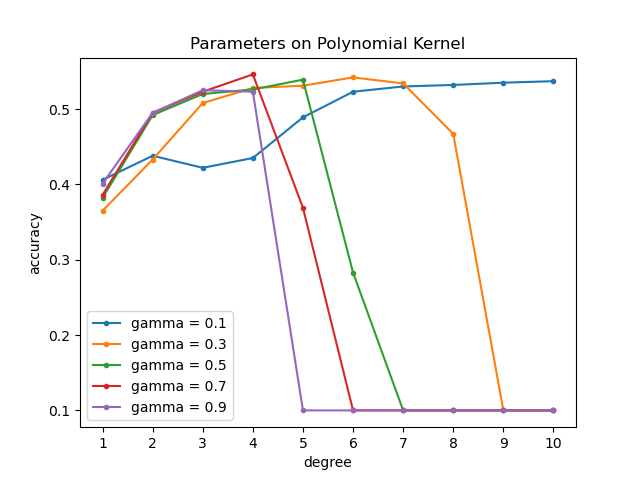
\includegraphics[width=0.5\textwidth]{Figure_1.png}
  \caption{Result of Polynomial Kernel}
  \label{fig:poly}
\end{figure}\\
We can see from figure 4 that for a fixed $\gamma$, the accuracy drops to 0.1 as the degree increases and the larger of the $\gamma$, the faster accuracy drops to 0.1. Meanwhile, we also know that when $\gamma=0.7$, degree=4, the accuracy reaches its maximal value 0.546.
\\Similarly, we repeat the ablation experiment with every kernel and then apply it on MNIST (original $28\times 28$)and CIFAR-10
(HOG features). The result on test set is shown in table $1$
\begin{table}[h!]
  \begin{center}
    \begin{tabular}{l|c|c} % <-- Alignments: 1st column left, 2nd middle and 3rd right, with vertical lines in between
      \textbf{Kernel} & \textbf{MNIST} & \textbf{CIFAR-10}\\
      \hline
      Linear & 0.899 & 0.450\\
      Polynomial & 0.939 & \textbf{0.546}\\
      Gaussian & \textbf{0.942} & 0.533\\
      Sigmoid & 0.782 & 0.384\\
    \end{tabular}
    \caption{Result of Different Kernel}
  \end{center}
\end{table}
The result of Sigmoid kernel, Linear kernel as well as Gaussian kernel on CIFAR-10 and MNIST is shown in figure \ref{fig:sigmoid}, figure \ref{fig:linear} and figure \ref{fig:gaussian}. Additionally, we found the efficiency of Gaussian kernel is extremely low compared with other three kernels due to its complex calculation. The efficiency of the three kernels is similar and all higher than the efficiency of Gaussian kernel. The efficiency on MINIST is overall higher than the efficiency on CIFAR-10 due to its small size of only $28\times 28$ compared with HOG features of CIFAR-10 with a size of $1568\times 1$.
\begin{figure}[htb]
  \centering
  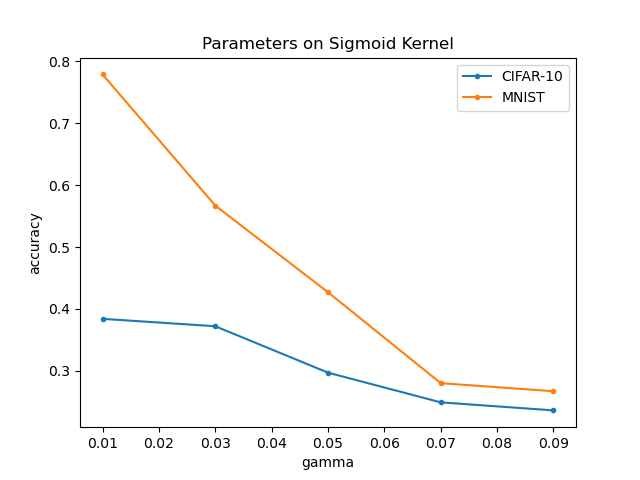
\includegraphics[width=0.5\textwidth]{Sigmoid.png}
  \caption{Result of Sigmoid Kernel}
  \label{fig:sigmoid}
\end{figure}
\begin{figure}[htb]
  \centering
  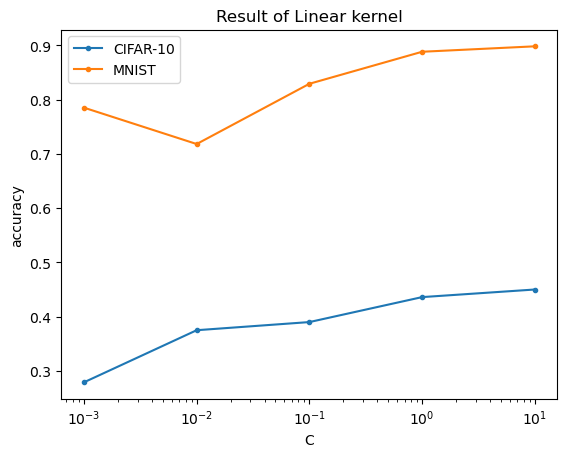
\includegraphics[width=0.5\textwidth]{Linear.png}
  \caption{Result of Linear Kernel}
  \label{fig:linear}
\end{figure}
\begin{figure}[htb]
  \centering
  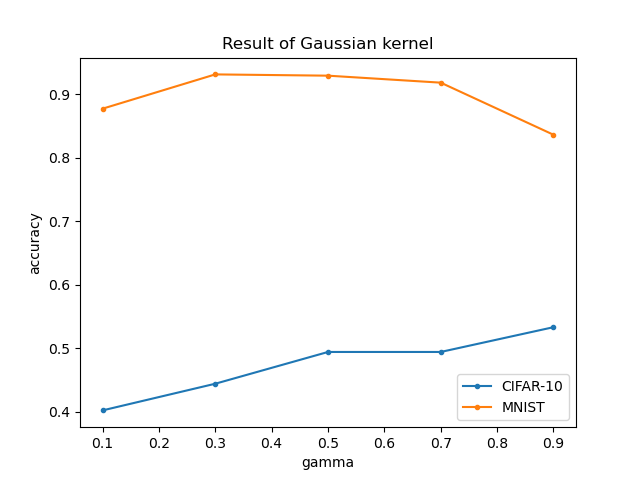
\includegraphics[width=0.5\textwidth]{Gaussian.png}
  \caption{Result of Gaussian Kernel}
  \label{fig:gaussian}
\end{figure}

\subsection{SVM With Multiple Kernels}
When SVM combines multiple kernels together, it is capable to various complex situations. The type of kernel and its weights as well as each kernel's parameters become the key to this method.\\
In our experiment, we mainly focus on the combination of different kernels with each weight determined by the above-mentioned algorithm, and test their accuracy on both MNIST and CIFAR-10. The parameters we choose are according to the experiment of single kernel and select the parameters with which single kernel performs well. The result on MNIST 
 test set is shown in table $2$ and the result on CIFAR-10 test set is shown in table $3$.
\begin{table}[h!]
  \begin{center}
    \begin{tabular}{c|c|c|c|c}
      \textbf{Line} & \textbf{Poly} & \textbf{Gaus} & \textbf{Sigm} & \textbf{Accuray}\\
      \hline
      \checkmark & & & \checkmark & 0.872\\
      \checkmark & \checkmark & & & 0.912\\
      \checkmark & & \checkmark & & 0.915\\
       & \checkmark & & \checkmark & 0.886\\
       & \checkmark & \checkmark & & \textbf{0.927}\\
       & & \checkmark & \checkmark & 0.876\\
      \checkmark & \checkmark & \checkmark & \checkmark & 0.862
    \end{tabular}
    \caption{Multiple Kernels on MNIST}
  \end{center}
\end{table}
\begin{table}[h!]
  \begin{center}
    \begin{tabular}{c|c|c|c|c}
      \textbf{Line} & \textbf{Poly} & \textbf{Gaus} & \textbf{Sigm} & \textbf{Accuray}\\
      \hline
      \checkmark & & & \checkmark & 0.301\\
      \checkmark & \checkmark & & & 0.348\\
      \checkmark & & \checkmark & & 0.324\\
       & \checkmark & & \checkmark & 0.407\\
       & \checkmark & \checkmark & & 0.355\\
       & & \checkmark & \checkmark & 0.377\\
      \checkmark & \checkmark & \checkmark &  & 0.363\\
      \checkmark & \checkmark &  & \checkmark & 0.342\\
       & \checkmark & \checkmark & \checkmark & \textbf{0.465}\\
       \checkmark &  & \checkmark & \checkmark & 0.366\\
      \checkmark & \checkmark & \checkmark & \checkmark & 0.42
    \end{tabular}
    \caption{Multiple Kernels on CIFAR-10}
  \end{center}
\end{table}
\\Notice that the two table fix the decay parameter $d=0.3$, in order to know effect of $d$, an ablation experiment is performed. By changing different $d$, test the accuracy of some combinations of 4 kernels on CIFAR-10. The result is shown in figure \ref{fig:decay}, notice that $S\& L\& G\& P$ means the combination of Sigmoid, Linear, Gaussian and Polynomial kernels.
\begin{figure}[htb]
  \centering
  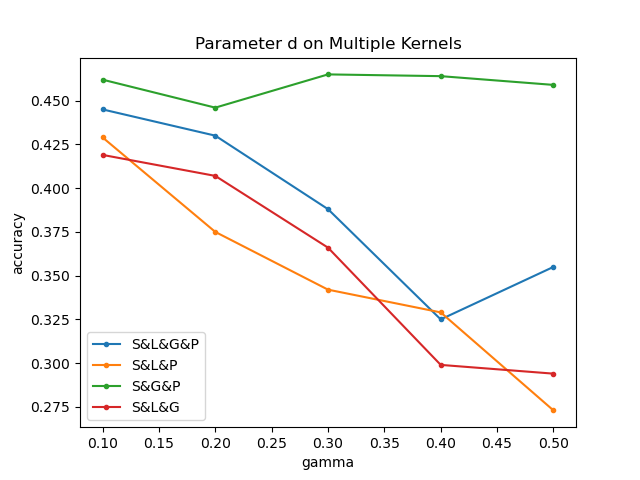
\includegraphics[width=0.5\textwidth]{decay.png}
  \caption{$d$ on Multiple Kernels}
  \label{fig:decay}
\end{figure}
\\From the result of table 2, table 3 and figure 7, we know that when $d=0.1$, the algorithm performs well and the combination of Sigmoid, Linear, Gaussian and Polynomial performs best. Additionally, the accuracy is stable when $d$ changes. However, the accuracy shows that the combination of multiple kernels may performs even worse than the single kernel with our method.\\
The efficiency is similar to single kernel: The efficiency of Gaussian kernel is extremely low and the efficiency of any combination with Gaussian kernel is much lower than the combination without Gaussian kernel.


\section{Conclusion}
In the project, we focus on SVM algorithm and extend the algorithm to classify multiple labels and study the algorithm of multiple kernels and the influence of different combinations and different parameters based on MNIST and CIFAR-10. In SVM with single kernel, we study the parameters and the type of kernels and found that Gaussian kernel and Polynomial kernel performs well. In SVM with multiple kernels, study the combination of kernels and the decay parameter and found that the combination of Sigmoid, Gaussian and Polynomial kernels performs well. And is less likely to be influenced by the decay parameter d. Until now, the problem of multiple kernels still lacks an optimal solution and is still waiting for an ideal method.

\begin{thebibliography}{99}  

\bibitem{ref1}王行甫,俞璐.混合核函数中权重求解方法.计算机系统应用,2015,24(4):129-133
\bibitem{ref2}https://zhuanlan.zhihu.com/p/29212107
\end{thebibliography}


\end{document}
